\documentclass[11pt]{amsart}
\usepackage[a4paper,margin=2.7cm]{geometry}
\usepackage{amssymb}
\usepackage{tikz}
\usepackage[hidelinks]{hyperref}
\newtheorem{theorem}{Theorem}
\newtheorem{proposition}{Proposition}[section]
\newtheorem{lemma}[proposition]{Lemma}
\newtheorem{corollary}[proposition]{Corollary}
\theoremstyle{definition}
\newtheorem{definition}[proposition]{Definition}
\theoremstyle{remark}
\newtheorem{remark}[proposition]{Remark}
\numberwithin{equation}{section}

\newcommand{\cF}{\mathsf F}
\newcommand{\cG}{\mathsf G}
\newcommand{\cT}{\mathsf T}

\title[The Hofstadter--Conway sequence and its alternating variant]{A comparison theorem for the Hofstadter--Conway\\ \$10{,}000 sequence and its alternating variant}
\author{Vamshi Jandhyala}
\date{Preprint, version 1, 8 October 2026. Not peer reviewed.}
\subjclass[2020]{11B37, 05A15}
\keywords{Hofstadter--Conway sequence, meta-Fibonacci recurrence, nested recurrence, Dyck path}

\begin{document}

\begin{abstract}
Let $c$ be the Hofstadter--Conway \$10{,}000 sequence, $c(n)=c(c(n-1))+c(n-c(n-1))$, and let $s$ be the sequence defined by $s(n)=n-s(s(n-1))-s(n-s(n-1))$, both with initial values $1,1$ (OEIS A004001 and A287422). Alkan conjectured in 2020 that $|s(n)-n/2|\le c(n)-n/2$ for every $n\ge1$. We prove the conjecture. On each dyadic block $[2^k,2^{k+1}]$ both sequences are encoded by Dyck words, and the words for the next block are produced by two explicit threshold operators. The proof rests on a two-step domination lemma for symmetric Dyck words, which compares the operators after a small perturbation at the centre of the word.
\end{abstract}

\maketitle

\noindent\emph{Status of this preprint.} Every result of this paper is formally verified in Lean~4 (Section~\ref{sec:remarks}), using only Lean's standard axioms. This version has not yet been independently reviewed.

\section{Introduction}

The Hofstadter--Conway sequence
\[
c(1)=c(2)=1,\qquad c(n)=c(c(n-1))+c(n-c(n-1))\quad(n\ge3)
\]
is sequence A004001 of the OEIS~\cite{A004001}. Conway stated that $c(n)/n\to\frac12$ and offered a prize for a quantitative form of this statement, which was claimed by Mallows~\cite{Mallows}. Kubo and Vakil~\cite{KV} gave a detailed analysis of its structure on the dyadic blocks $[2^k,2^{k+1}]$, on each of which $c(n)-\frac n2$ traces a positive arch.

Alkan~\cite{A287422} introduced the companion sequence
\[
s(1)=s(2)=1,\qquad s(n)=n-s(s(n-1))-s(n-s(n-1))\quad(n\ge3),
\]
studied with related recursions in~\cite{AA}. Its graph of $s(n)-\frac n2$ also consists of arches over the dyadic blocks, but their signs alternate. In a MathOverflow question~\cite{MO} he conjectured, after checking all $n\le2^{32}$, that the arches of $s$ never rise above those of $c$.

\begin{theorem}\label{thm:main}
For every integer $n\ge1$,
\[
\Bigl|\,s(n)-\frac n2\,\Bigr|\le c(n)-\frac n2 .
\]
\end{theorem}

Equivalently, $n-c(n)\le s(n)\le c(n)$ for all $n$.

\subsection*{Outline} Encode the increments of $c$ on the block $[2^k,2^{k+1}]$ as a binary word $w_k$ of length $2^k$, and do the same for $s$, complementing the word on blocks where $s$ lies below $n/2$; call the result $v_k$. Section~\ref{sec:ops} defines two operators $\cF$ and $\cG$ that double the length of a Dyck word, and Section~\ref{sec:blocks} shows that $w_{k+1}=\cF(w_k)$ while $v_{k+1}$ is $\cF(v_k)$ or $\cG(v_k)$ according to the parity of $k$. Theorem~\ref{thm:main} becomes the statement that the lattice path of $v_k$ never rises above that of $w_k$. Plain induction fails because $\cG$ can overtake $\cF$ in one step. The remedy, in Section~\ref{sec:lemma}, is to carry a stronger hypothesis through two steps at once: $v_k$ lies below a perturbation $\cT(w_k)$ of $w_k$ that lowers its path by one level away from the ends. The key lemma (Lemma~\ref{lem:key}) holds for Dyck words that are symmetric under reversal and complement, and all the words $w_k$ have this symmetry. Figure~\ref{fig:k5} shows the three paths for $k=5$.

\begin{figure}[ht]
\centering
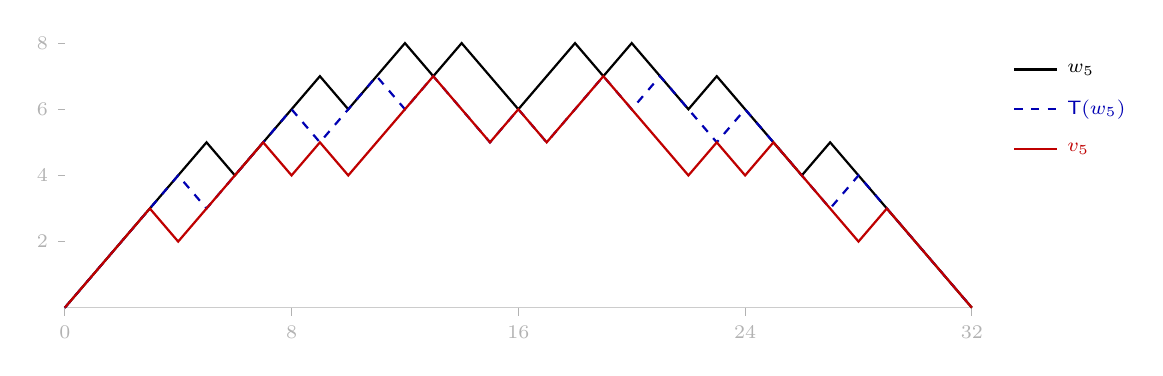
\begin{tikzpicture}[xscale=0.36,yscale=0.42]
\draw[gray!40] (0,0) -- (32,0);
\foreach \x in {0,8,16,24,32} {\draw[gray!60] (\x,0) -- (\x,-0.25) node[below,font=\scriptsize] {\x};}
\foreach \y in {2,4,6,8} {\draw[gray!60] (0,\y) -- (-0.25,\y) node[left,font=\scriptsize] {\y};}
\draw[thick,black] plot coordinates {(0,0) (1,1) (2,2) (3,3) (4,4) (5,5) (6,4) (7,5) (8,6) (9,7) (10,6) (11,7) (12,8) (13,7) (14,8) (15,7) (16,6) (17,7) (18,8) (19,7) (20,8) (21,7) (22,6) (23,7) (24,6) (25,5) (26,4) (27,5) (28,4) (29,3) (30,2) (31,1) (32,0)};
\draw[thick,dashed,blue!70!black] plot coordinates {(0,0) (1,1) (2,2) (3,3) (4,4) (5,3) (6,4) (7,5) (8,6) (9,5) (10,6) (11,7) (12,6) (13,7) (14,6) (15,5) (16,6) (17,5) (18,6) (19,7) (20,6) (21,7) (22,6) (23,5) (24,6) (25,5) (26,4) (27,3) (28,4) (29,3) (30,2) (31,1) (32,0)};
\draw[thick,red!75!black] plot coordinates {(0,0) (1,1) (2,2) (3,3) (4,2) (5,3) (6,4) (7,5) (8,4) (9,5) (10,4) (11,5) (12,6) (13,7) (14,6) (15,5) (16,6) (17,5) (18,6) (19,7) (20,6) (21,5) (22,4) (23,5) (24,4) (25,5) (26,4) (27,3) (28,2) (29,3) (30,2) (31,1) (32,0)};
\begin{scope}[shift={(33.5,6)},font=\scriptsize]
\draw[thick,black] (0,1.2) -- (1.5,1.2) node[right] {$w_5$};
\draw[thick,dashed,blue!70!black] (0,0) -- (1.5,0) node[right] {$\cT(w_5)$};
\draw[thick,red!75!black] (0,-1.2) -- (1.5,-1.2) node[right] {$v_5$};
\end{scope}
\end{tikzpicture}
\caption{Heights of the block words for $k=5$, that is, $2c(n)-n$ (black) and $|2s(n)-n|$ (red) for $32\le n\le64$, plotted against $n-32$. The dashed path is $\cT(w_5)$, which lies between them, as the induction requires.}
\label{fig:k5}
\end{figure}

As by-products, the construction shows that $s$ is well defined and \emph{slow} (its increments are $0$ or $1$), that $s(2^k)=2^{k-1}$, and that $s(n)-\frac n2$ is non-negative on $[2^k,2^{k+1}]$ for even $k$ and non-positive for odd $k$.

\section{Dyck words and two threshold operators}\label{sec:ops}

\subsection{Words} A binary word $u=u_1\cdots u_L$ has prefix counts $P_u(i)=u_1+\dots+u_i$, with $P_u(0)=0$. We write $P$ when $u$ is clear. Throughout, $L$ is even and $m=L/2$. The word is a \emph{Dyck word} if $2P(i)\ge i$ for all $i$ and $P(L)=m$; its \emph{height} at $i$ is $2P(i)-i$. It is \emph{irreducible} if $2P(i)>i$ for $0<i<L$, and \emph{symmetric} if $u_{L+1-i}=1-u_i$ for all $i$. For words of equal length we write $u\le v$ if $P_u(i)\le P_v(i)$ for every $i$. For a Dyck word, $u_1=1$ and $u_L=0$.

\begin{lemma}\label{lem:sym}
A word $u$ of length $L=2m$ with $P(L)=m$ is symmetric if and only if
\begin{equation}\label{eq:sym}
P(L-i)=m-i+P(i)\qquad(0\le i\le L).
\end{equation}
\end{lemma}

\begin{proof}
If $u$ is symmetric, then $P(L)-P(L-i)=\sum_{s=1}^{i}u_{L+1-s}=\sum_{s=1}^i(1-u_s)=i-P(i)$. Conversely, taking differences of \eqref{eq:sym} at $i-1$ and $i$ gives $u_{L+1-i}=1-u_i$.
\end{proof}

\subsection{The operators} Let $u$ be a Dyck word of length $L$. For $0\le j\le 2L$ let $I_j=[\max(0,j-L),\min(j,L)]\cap\mathbb Z$ and define
\[
d_j(a)=a-P(a)-P(j-a)\qquad(a\in I_j).
\]
Set
\[
A(j)=\min\{a\in I_j: d_j(a)\ge0\},\qquad B(j)=\max\{a\in I_j: d_j(a)\le0\}.
\]
Lemma~\ref{lem:ops} shows that $A$ and $B$ are the prefix counts of Dyck words of length $2L$, which we call $\cF(u)$ and $\cG(u)$.

The definition comes from the recurrences. When $u$ encodes $c$ on one dyadic block, the two earlier values that the recurrence for $c$ reads on the next block sit at positions $a=A(j-1)$ and $j-a$ of $u$, and~\eqref{eq:A} below is the recurrence itself (Proposition~\ref{prop:blocks}); $d_j(a)$ measures how far a candidate $a$ is from that consistency. For example, take $u=1100$, so $L=4$ and $P=0,1,2,2,2$. For $j=3$ the values $d_3(a)$, $a=0,1,2,3$, are $-2,-2,-1,1$, so $A(3)=3$ and $B(3)=2$; for $j=4$ they are $-2,-2,-2,0,2$, so $A(4)=B(4)=3$. Running over $j=0,\dots,8$ gives
\[
A=0,1,2,3,3,4,4,4,4,\qquad B=0,1,2,2,3,3,4,4,4,
\]
so $\cF(1100)=11101000$ and $\cG(1100)=11010100$. These are the block words $w_3$ and $v_3$ of $c$ and $s$ on $[8,16]$ (Section~\ref{sec:blocks}).

\begin{lemma}\label{lem:ops}
Let $u$ be a Dyck word of length $L$.
\begin{enumerate}
\item Both thresholds exist; $d_j(A(j))\in\{0,1\}$ and $d_j(B(j))\in\{-1,0\}$.
\item $A(j),B(j)\ge j/2$, and $A(2L)=B(2L)=L$.
\item For $1\le j\le 2L$, with the convention $P(L+1)=P(L)$,
\begin{align}
A(j)&=P(A(j-1))+P(j-A(j-1)),\label{eq:A}\\
B(j)&=P(B(j-1)+1)+P(j-1-B(j-1)).\label{eq:B}
\end{align}
All arguments of $P$ lie in $[0,L]$, except that $B(j-1)+1$ may equal $L+1$.
\item $A(j)-A(j-1)$ and $B(j)-B(j-1)$ lie in $\{0,1\}$. Hence $\cF(u)$ and $\cG(u)$ are Dyck words of length $2L$.
\item If $A(j)=a$, $d_j(a)=1$ and $a-1\in I_j$, then $u_a=0$.
\end{enumerate}
\end{lemma}

\begin{proof}
(1) For $a,a+1\in I_j$,
\begin{equation}\label{eq:inc}
d_j(a+1)-d_j(a)=1-u_{a+1}+u_{j-a}\in\{0,1,2\},
\end{equation}
so $d_j$ is non-decreasing. At the left end of $I_j$, $d_j(0)=-P(j)\le0$ if $j\le L$, and $d_j(j-L)=(j-L)-P(j-L)-m\le\frac{j-L}{2}-m\le0$ if $j>L$, using $P(i)\ge i/2$. At the right end, $d_j(j)=j-P(j)\ge0$ if $j\le L$, and $d_j(L)=m-P(j-L)\ge0$ if $j>L$. So both thresholds exist. If $A(j)$ is the left end of $I_j$ then $d_j(A(j))=0$; otherwise its predecessor has a negative value and \eqref{eq:inc} gives $d_j(A(j))\le1$. The claim for $B$ is symmetric.

(2) If $a<j/2$ then $d_j(a)\le a-\frac a2-\frac{j-a}2=a-\frac j2<0$, so $A(j)\ge j/2$. For $a=\lceil j/2\rceil\in I_j$ the same estimate gives $d_j(a)\le\frac12$, hence $d_j(a)\le0$ and $B(j)\ge\lceil j/2\rceil$. Finally $I_{2L}=\{L\}$.

(3) Let $a=A(j-1)$ and $e=d_{j-1}(a)$. By (2), $a\ge\frac{j-1}2>j-1-L$, so $a\ge j-L$ and $a\in I_j$; also $1\le j-a\le L$. Directly from the definition,
\begin{equation}\label{eq:shift}
d_j(x)=d_{j-1}(x)-u_{j-x},\qquad d_j(x+1)=d_{j-1}(x)+1-u_{x+1},
\end{equation}
so $d_j(x)<0$ for $x<a$ in $I_j$, and $d_j(a+1)\ge0$ when $a+1\in I_j$. Hence $A(j)\in\{a,a+1\}$. The right side of \eqref{eq:A} equals $P(a)+P(j-1-a)+u_{j-a}=a-e+u_{j-a}$.

If $e=0$ and $u_{j-a}=0$, then $d_j(a)=0$ and $A(j)=a$. If $e=0$ and $u_{j-a}=1$, then $d_j(a)=-1$, so $A(j)=a+1$ (here $a<L$, since $a=L$ would force $P(j-1-L)=m$ and then $P(j-L)=m+1$). If $e=1$, then $a$ is not the left end of $I_{j-1}$, and $d_{j-1}(a-1)<0$ together with \eqref{eq:inc} forces $u_a=0$ and $u_{j-a}=1$; then $d_j(a)=0$ and $A(j)=a$. In every case $A(j)=a-e+u_{j-a}$.

For \eqref{eq:B}, let $b=B(j-1)$ and $e=d_{j-1}(b)\in\{-1,0\}$. As before $b\ge j-L$ and $0\le j-1-b\le L$. If $e=-1$, then $b$ is not the right end of $I_{j-1}$, so $d_{j-1}(b+1)>0$ and \eqref{eq:inc} forces $u_{b+1}=0$; then $d_j(b+1)=d_{j-1}(b)+1=0$ by \eqref{eq:shift}, while $d_j(x)\ge d_{j-1}(x-1)>0$ for $x>b+1$, so $B(j)=b+1=P(b+1)+P(j-1-b)$. If $e=0$ and $b<L$ with $u_{b+1}=1$, the same computation gives $d_j(b+1)=0$ and $B(j)=b+1$. If $e=0$ and either $b=L$ or $u_{b+1}=0$, then $B(j)=b$, because $d_j(b)\le d_{j-1}(b)=0$ and $d_j(b+1)=1$ when $b<L$. In each case $B(j)=b-e+u_{b+1}$ with $u_{L+1}:=0$, which is \eqref{eq:B}.

(4) follows from (3) and its proof, and with (2) it shows that $A$ and $B$ are prefix counts of Dyck words.

(5) We have $d_j(a-1)<0$, so by \eqref{eq:inc} $1-u_a+u_{j-a+1}\ge2$, giving $u_a=0$.
\end{proof}

\begin{lemma}\label{lem:props}
Let $u,v$ be Dyck words of length $L$.
\begin{enumerate}
\item \emph{Monotonicity.} If $u\le v$ then $\cF(u)\le\cF(v)$ and $\cG(u)\le\cG(v)$.
\item If $u$ is irreducible, so is $\cF(u)$.
\item If $u$ is symmetric, so are $\cF(u)$ and $\cG(u)$.
\end{enumerate}
\end{lemma}

\begin{proof}
(1) If $P_u\le P_v$ then $d^u_j(a)\ge d^v_j(a)$ for every $a$, so both thresholds for $u$ are at most those for $v$.

(2) Suppose $2A(j)=j$ with $0<j<2L$, and put $a=j/2$, so $0<a<L$. Then $0\le d_j(a)=a-2P(a)$, contradicting irreducibility of $u$.

(3) Let $a'=L-j+a$. The map $a\mapsto a'$ is an increasing bijection from $I_j$ to $I_{2L-j}$, and by \eqref{eq:sym},
\[
d_{2L-j}(a')=a'-P(L-(j-a))-P(L-a)=a-P(a)-P(j-a)=d_j(a).
\]
Hence $A(2L-j)=L-j+A(j)$ and $B(2L-j)=L-j+B(j)$, which is \eqref{eq:sym} for the outputs, whose half-length is $L$.
\end{proof}

\subsection{The central perturbation} For a symmetric irreducible Dyck word $u$ of length $L=2m\ge4$ define
\[
\cT(u)=u_2u_3\cdots u_m\;b\;(1-b)\;u_{m+1}\cdots u_{L-1},\qquad b=1-u_m.
\]
The first $1$ and the last $0$ of $u$ are removed and a complementary pair is inserted at the centre. When the centre of $u$ is a peak ($u_mu_{m+1}=10$) it becomes a valley, and vice versa. Away from the centre, the path of $\cT(u)$ is the path of $u$ lowered by one level.

\begin{lemma}\label{lem:T}
Let $u$ be a symmetric irreducible Dyck word of length $L=2m\ge4$, and $u'=\cT(u)$. Then $u'$ is a symmetric Dyck word and $u'\le u$. More precisely, $\delta(i)=P_u(i)-P_{u'}(i)$ is given by
\begin{equation}\label{eq:delta}
\delta(i)=\begin{cases}1-u_{i+1},&0\le i<m,\\ u_m,&i=m,\\ u_i,&m<i\le L.\end{cases}
\end{equation}
\end{lemma}

\begin{proof}
Formula \eqref{eq:delta} is read off from the definition, using $u_1=1$. Since $\delta\ge0$, $u'\le u$. The two central letters are complementary and the others are matched by the symmetry of $u$, so $u'$ is symmetric. The height of $u'$ is $h(i+1)-1$ for $i<m$ and $h(i-1)-1$ for $i>m$, where $h$ is the height of $u$; these are non-negative because $h>0$ at interior points and $h(L)=0$. At the centre the height is $h(m)-2u_m$, which is non-negative because $h(m)=h(m-1)+1\ge2$ when $u_m=1$.
\end{proof}

\section{The symmetric two-step lemma}\label{sec:lemma}

\begin{lemma}[Key lemma]\label{lem:key}
For every symmetric irreducible Dyck word $u$ of length $L=2m\ge4$,
\[
\cG(\cF(\cT(u)))\le\cT(\cF(\cF(u))).
\]
\end{lemma}

The right side is defined because $\cF(\cF(u))$ is symmetric and irreducible by Lemma~\ref{lem:props}.

\begin{proof}
Let $u'=\cT(u)$ with prefix counts $P'$ and $\delta=P-P'$ as in \eqref{eq:delta}. Let $H$ and $K$ be the prefix counts of $\cF(u)$ and $\cF(u')$; by Lemma~\ref{lem:T} and monotonicity, $K\le H$. Let $W$ and $Z$ be the prefix counts of $w=\cF(\cF(u))$ and $\cG(\cF(u'))$. These are symmetric words of length $4L$; put $M=2L$, the midpoint. For $j\le M$ the index set in the definition of $W(j)$ and $Z(j)$ is $[0,j]$.

\smallskip\noindent\emph{Step 1: a midpoint identity.} Let $a=W(M)$. By Lemma~\ref{lem:sym} for $\cF(u)$, $H(M-a)=L-a+H(a)$, so the threshold value at $a$ is $a-H(a)-H(M-a)=2a-L-2H(a)$. It is even and lies in $\{0,1\}$, so it is $0$. Hence $H(a)=a-m$ and
\[
H(M-W(M))=m.
\]
Since $j-W(j)$ is non-decreasing in $j$ and $H$ is non-decreasing,
\begin{equation}\label{eq:mid}
H(j-W(j))\le m\qquad(0\le j\le M).
\end{equation}

\smallskip\noindent\emph{Step 2: the contact claim.} We show that if $0\le j\le M$ and $Z(j)=W(j)$, then $w_{j+1}=1$.

Put $a=W(j)=Z(j)$ and $q=j-a$. By Lemma~\ref{lem:ops}(1) for $W$ and for $Z$, and $K\le H$,
\[
0\le a-H(a)-H(q)\le a-K(a)-K(q)\le0.
\]
So equality holds throughout, and with $K\le H$ this gives $H(a)=K(a)$ and $H(q)=K(q)=:y$. Put $z=q-y$. By Lemma~\ref{lem:ops}(2) applied to $H$, $y\ge q/2$, so $0\le z\le y$, and $q\le j/2\le L$. By \eqref{eq:mid}, $y\le m$.

By \eqref{eq:A} for the outer operator, $W(j+1)=H(a)+H(q+1)$, so $w_{j+1}=H(q+1)-H(q)$, the letter of $\cF(u)$ at position $q+1$. By \eqref{eq:A} for the inner operator, $H(q+1)=P(y)+P(z+1)$. Writing
\[
e=y-P(y)-P(z),\qquad e'=y-P'(y)-P'(z),
\]
these are the threshold values of $y=H(q)$ for $u$ and of $y=K(q)$ for $u'$, so $e,e'\in\{0,1\}$ and
\begin{equation}\label{eq:ee}
e'=e+\delta(y)+\delta(z),\qquad w_{j+1}=u_{z+1}-e.
\end{equation}

Suppose $w_{j+1}=0$, so $u_{z+1}=e$. If $y=0$ then $q=0$ and $w_{j+1}=H(1)=1$, a contradiction; so $y\ge1$. If $z=m$ then $y=m$ and $q=L$, and $H(L)=m$ says that $\cF(u)$ has height $0$ at the interior point $L$, contradicting Lemma~\ref{lem:props}(2); so $z<m$. By \eqref{eq:delta}, $\delta(z)=1-u_{z+1}=1-e$, and \eqref{eq:ee} gives $e'=1+\delta(y)$. As $e'\le1$, we get $e'=1$ and $\delta(y)=0$.

Now $\delta(y)=0$ says $u'_y=1$: for $y<m$ it gives $u_{y+1}=1$ and $u'_y=u_{y+1}$, and for $y=m$ it gives $u_m=0$, so $u'_m=1-u_m=1$. On the other hand, $y=K(q)$ is the first threshold for $u'$ at index $q$, its value is $e'=1$, and $y-1\in[0,q]=I_q$. Lemma~\ref{lem:ops}(5) gives $u'_y=0$. This contradiction proves the claim.

\smallskip\noindent\emph{Step 3: $Z\le W$.} Both start at $0$ and have increments $0$ or $1$. If $Z(j)>W(j)$ for some $j\le M$, take the least such $j$; then $Z(j-1)=W(j-1)$ and $w_j=0$, contradicting Step~2. So $Z\le W$ on $[0,M]$, and by Lemma~\ref{lem:sym} applied to both words, $Z(4L-j)-W(4L-j)=Z(j)-W(j)$, so $Z\le W$ everywhere.

\smallskip\noindent\emph{Step 4: domination by $\cT(w)$.} By \eqref{eq:delta} applied to $w$, the prefix count of $\cT(w)$ is $W(i)-1+w_{i+1}$ for $i<M$ and $W(M)-w_M$ at $i=M$. For $i<M$: if $w_{i+1}=1$ this is $W(i)\ge Z(i)$; if $w_{i+1}=0$, Step~2 gives $Z(i)\ne W(i)$, so $Z(i)\le W(i)-1$. At $i=M$: if $w_M=0$ the bound is $Z(M)\le W(M)$; if $w_M=1$ then $w_{M+1}=0$ by symmetry, and Step~2 again gives $Z(M)\le W(M)-1$. For $i>M$ the bound follows from the case $4L-i<M$, since $\cT(w)$ and $\cG(\cF(u'))$ are both symmetric.
\end{proof}

\begin{remark}
Symmetry enters through the midpoint identity, which gives the bound $y\le m$ in Step~2. Without symmetry both fail. Among irreducible Dyck words $u$, the identity $H(M-W(M))=m$ first fails at length $12$ (for $3$ words), and the bound~\eqref{eq:mid} first fails at length $16$ (for $8$ words).
\end{remark}

\section{The block words of \texorpdfstring{$c$}{c} and \texorpdfstring{$s$}{s}}\label{sec:blocks}

For $k\ge1$ and $L=2^k$ let $w_k$ be the word of increments $c(L+t)-c(L+t-1)$, $1\le t\le L$. Let $v_k$ be the word of increments of $s$ on the same range when $k$ is even, and the complement of that word when $k$ is odd.

\begin{proposition}\label{prop:blocks}
The sequence $s$ is well defined for all $n$, and for every $k\ge1$ the words $w_k,v_k$ are Dyck words with
\[
w_1=v_1=10,\qquad w_{k+1}=\cF(w_k),\qquad v_{k+1}=\begin{cases}\cF(v_k),&k\text{ odd},\\ \cG(v_k),&k\text{ even}.\end{cases}
\]
Moreover, for $L=2^k$ and $0\le t\le L$,
\begin{equation}\label{eq:blocks}
c(L+t)=\tfrac L2+P_{w_k}(t),\qquad s(L+t)=\begin{cases}\tfrac L2+P_{v_k}(t),&k\text{ even},\\ \tfrac L2+t-P_{v_k}(t),&k\text{ odd}.\end{cases}
\end{equation}
\end{proposition}

\begin{proof}
Define words $\bar w_k,\bar v_k$ by the recursions in the statement, and define $\bar c,\bar s$ on $[2,\infty)$ by \eqref{eq:blocks} with these words. Since each word is Dyck, the two formulas at $n=2L$ (the end of block $k$ and the start of block $k+1$) both give $L$, so $\bar c,\bar s$ are well defined. We show that $\bar c,\bar s$, extended by $\bar c(1)=\bar s(1)=1$, satisfy the defining recurrences, with every argument on the right in $[1,n-1]$. Strong induction on $n$ then gives $\bar c=c$ and $\bar s=s$, and shows that $s$ is well defined. The values $1,2,2$ of $c$ and $1,1,2$ of $s$ on $[2,4]$ agree with block $1$.

Fix $k\ge1$, $L=2^k$, and $n=2L+j$ with $1\le j\le 2L$. Let $u$ be the parent word ($\bar w_k$ or $\bar v_k$) with prefix count $P$ and thresholds $A,B$.

\emph{Conway, or $s$ with $k$ odd.} Here $\bar c(2L+j)=L+A(j)$, and for odd $k$ also $\bar s(2L+j)=L+A(j)$, each with $A$ computed from its own parent word. Let $r=A(j-1)$; then $r\in[0,L]$ and $j-r\in[1,L]$ by the proof of Lemma~\ref{lem:ops}(3), so both $L+r$ and $L+j-r$ lie in block $k$ and are less than $n$. For $c$,
\[
\bar c(\bar c(n-1))+\bar c(n-\bar c(n-1))=\bar c(L+r)+\bar c(L+j-r)=L+P(r)+P(j-r)=L+A(j)
\]
by \eqref{eq:A}. For $s$ with $k$ odd, the parent block is given by the second case of \eqref{eq:blocks}, and
\[
n-\bar s(L+r)-\bar s(L+j-r)=2L+j-\bigl(L+j-P(r)-P(j-r)\bigr)=L+A(j).
\]

\emph{$s$ with $k$ even.} Here $\bar s(2L+j)=L+j-B(j)$ and the parent is $\bar s(L+t)=\frac L2+P(t)$. Let $r=B(j-1)$, so $\bar s(n-1)=L+\rho$ with $\rho=j-1-r\in[0,L]$, and $n-\bar s(n-1)=L+r+1$. If $r<L$ this lies in block $k$ and $\bar s(L+r+1)=\frac L2+P(r+1)$. If $r=L$, then $j\ge2$ and $L+r+1=2L+1$ is an earlier point of block $k+1$, where $\bar s(2L+1)=L+1-B(1)=L=\frac L2+P(L+1)$, because $B(1)=1$ for a Dyck word. In both cases, by \eqref{eq:B},
\[
n-\bar s(L+\rho)-\bar s(L+r+1)=2L+j-L-P(j-1-r)-P(r+1)=L+j-B(j).
\]
All arguments are at least $1$, and $L+r+1<n$ because $r=L$ forces $j\ge2$.

The induction runs over $j$ within each block and over $k$. The words $\bar w_k,\bar v_k$ are Dyck by Lemma~\ref{lem:ops}(4), so they are the increment words described before the proposition.
\end{proof}

\begin{corollary}\label{cor:heights}
For $L=2^k$ and $0\le t\le L$,
\[
2c(L+t)-(L+t)=2P_{w_k}(t)-t,\qquad (-1)^k\bigl(2s(L+t)-(L+t)\bigr)=2P_{v_k}(t)-t\ge0.
\]
In particular $s(2^k)=c(2^k)=2^{k-1}$, the sequence $s$ is slow, and $s(n)-\frac n2$ has sign $(-1)^k$ or vanishes on $[2^k,2^{k+1}]$. Theorem~\ref{thm:main} for $n\ge2$ is equivalent to $v_k\le w_k$ for all $k\ge1$.
\end{corollary}

\begin{proof}
Substitute \eqref{eq:blocks}. The heights of the Dyck words $w_k,v_k$ are non-negative.
\end{proof}

\begin{lemma}\label{lem:wsym}
Every $w_k$ is symmetric and irreducible, and every $v_k$ is symmetric.
\end{lemma}

\begin{proof}
The word $10$ is symmetric and irreducible. Apply Lemma~\ref{lem:props}(2),(3).
\end{proof}

\section{Proof of Theorem~\ref{thm:main}}\label{sec:proof}

The first blocks are computed directly from \eqref{eq:A} and \eqref{eq:B}:
\[
w_2=v_2=1100,\qquad w_3=\cF(1100)=11101000,\qquad v_3=\cG(1100)=11010100.
\]
Deleting the first $1$ and the last $0$ of $w_3$ leaves $110100$, and inserting $10$ at its centre gives $\cT(w_3)=11010100=v_3$.

We prove $v_k\le\cT(w_k)$ for every odd $k\ge3$ by induction. The case $k=3$ is the equality above. If it holds for an odd $k$, then by monotonicity (Lemma~\ref{lem:props}(1)) and the key lemma (Lemma~\ref{lem:key}, applicable by Lemma~\ref{lem:wsym}),
\[
v_{k+2}=\cG(\cF(v_k))\le\cG(\cF(\cT(w_k)))\le\cT(\cF(\cF(w_k)))=\cT(w_{k+2}).
\]
For the even blocks between them, $v_{k+1}=\cF(v_k)\le\cF(\cT(w_k))\le\cF(w_k)=w_{k+1}$, using $\cT(w_k)\le w_k$ (Lemma~\ref{lem:T}). Together with $v_1=w_1$ and $v_2=w_2$, this gives $v_k\le w_k$ for all $k\ge1$, and Theorem~\ref{thm:main} for $n\ge2$ follows from Corollary~\ref{cor:heights}. For $n=1$ both sides equal $\frac12$. \qed


\section{Remarks}\label{sec:remarks}

\begin{enumerate}
\item The proof gives more than Theorem~\ref{thm:main}: for odd $k\ge3$ the path of $|2s(n)-n|$ on $[2^k,2^{k+1}]$ lies below the path of $2c(n)-n$ lowered by one level away from the ends, with the centre adjusted as in $\cT$ (Figure~\ref{fig:k5}).
\item The argument uses no enumeration. As an independent check, the conclusions of Lemmas~\ref{lem:ops}, \ref{lem:props}, \ref{lem:T} and~\ref{lem:key} were tested by computer on all $26{,}364$ symmetric irreducible Dyck words of length at most $34$, Proposition~\ref{prop:blocks} on every block up to $2^{20}$, and Theorem~\ref{thm:main} and Corollary~\ref{cor:heights} on all $n\le2^{20}$.
\item Every result of Sections~\ref{sec:ops} to~\ref{sec:proof} is also proved in the Lean~4 proof assistant with the Mathlib library: Lemma~\ref{lem:sym}, Lemmas~\ref{lem:ops} to~\ref{lem:key}, Proposition~\ref{prop:blocks} (including that $c$ and $s$ satisfy their recurrences with every argument in range), Corollary~\ref{cor:heights}, Lemma~\ref{lem:wsym}, Theorem~\ref{thm:main}, and the sharper statement of Remark~1. The proofs follow the paper; the base case $\cT(w_3)=v_3$ is checked by evaluation, as in Section~\ref{sec:proof}. They use no axioms beyond the standard ones, and sixteen deliberately altered statements and definitions are rejected by the proof checker. The Lean code and the verification program are at
\begin{center}\small\url{https://github.com/jvvk/mathematics/tree/main/hofstadter-conway-comparison}.\end{center}
\item Alkan also asked for a combinatorial description of $s$. Proposition~\ref{prop:blocks} gives one in the same spirit as the analysis of $c$ by Kubo and Vakil: each block of $s$ is obtained from the previous one by one of two explicit threshold operators, alternating with the parity of $k$.
\end{enumerate}

\section*{Acknowledgements}
The proofs, text, verification programs and Lean formalisation were developed with the AI assistants Claude (Anthropic) and Codex (OpenAI), under the author's direction. The author is responsible for the contents.

\begin{thebibliography}{9}
\bibitem{AA} A.~Alkan and O.~\"O.~Aybar, \emph{On families of solutions for meta-Fibonacci recursions related to Hofstadter--Conway \$10000 sequence}, in: Chaos and Complex Systems, Springer Proceedings in Complexity, Springer, Cham, 2020, pp.~149--158, \href{https://doi.org/10.1007/978-3-030-35441-1_14}{doi:10.1007/978-3-030-35441-1\_14}.
\bibitem{KV} T.~Kubo and R.~Vakil, \emph{On Conway's recursive sequence}, Discrete Math.\ 152 (1996), 225--252, \href{https://doi.org/10.1016/0012-365X(94)00303-Z}{doi:10.1016/0012-365X(94)00303-Z}.
\bibitem{Mallows} C.~L.~Mallows, \emph{Conway's challenge sequence}, Amer.\ Math.\ Monthly 98 (1991), 5--20, \href{https://doi.org/10.1080/00029890.1991.11995694}{doi:10.1080/00029890.1991.11995694}.
\bibitem{MO} A.~Alkan, \emph{A question related to the Hofstadter--Conway \$10000 sequence}, MathOverflow question 366772 (2020), \url{https://mathoverflow.net/q/366772}, accessed 8 October 2026.
\bibitem{A004001} OEIS Foundation Inc., \emph{The On-Line Encyclopedia of Integer Sequences}, sequence A004001, \url{https://oeis.org/A004001}, accessed 8 October 2026.
\bibitem{A287422} OEIS Foundation Inc., \emph{The On-Line Encyclopedia of Integer Sequences}, sequence A287422 (contributed by A.~Alkan, 2017), \url{https://oeis.org/A287422}, accessed 8 October 2026.
\end{thebibliography}

\end{document}
